\documentclass[letterpaper]{article}
\usepackage[vmargin=0.5in,hmargin=1in,includeheadfoot,head=0.5in,headsep=0.4602in,foot=0.5in,footskip=0.9602in]{geometry}
\usepackage{times}
\usepackage{sectsty}
\usepackage{titlesec}
\usepackage{tocloft}



\sectionfont{\fontsize{20}{22}\selectfont\bfseries} % Heading 1
\subsectionfont{\fontsize{16}{18}\selectfont} % Heading 2
\subsubsectionfont{\fontsize{14}{16}\selectfont} % Heading 3

\renewcommand{\cftsecfont}{\normalfont\fontsize{12}{14}\bfseries}
\renewcommand{\cftsubsecfont}{\normalfont\fontsize{12}{14}}
\renewcommand{\cftsecpagefont}{\normalfont\fontsize{12}{14}\bfseries}
\renewcommand{\cftsubsecpagefont}{\normalfont\fontsize{12}{14}}


\usepackage{calc,amsmath,amssymb,amsfonts}
\usepackage[T1]{fontenc}
\usepackage[english]{babel}
\usepackage{xcolor,longfbox,fancyhdr}
\usepackage{array,supertabular,hhline,enumitem,caption,hyperref}

\hypersetup{colorlinks=true,allcolors=black,pdfauthor=Alireza Foroutan}

\usepackage[pdftex]{graphicx}
\usepackage{tikz}



\begin{document}
	\begin{titlepage}
		\begin{center}
			
\includegraphics[width=3.1307in, height=1.2756in]{Picture2.png}
						
			\vspace{3cm}	
					
			    \textbf{\LARGE FOOTBALL MATCH RESULTS PREDICTOR}
								
			\vspace{3cm}
			
			\textbf{\Large Submitted by}
			\vspace{.5cm}		
			
			\textbf{\Large AMD}
							
			\vspace{0.5cm}				
				Dheeraj Parkash \\
				Muhammad Ahmed \\
				Alireza Foroutan				
			\vspace{1.5cm}
			
			\textbf{M1 Computer Science and Artificial Intelligence}\\
			Teacher: Enrico Formenti
			\vfill	
			\textbf{2023/2024}
			\end{center}
		\end{titlepage}
\clearpage

\newpage % Start on the sixth page
\tableofcontents
	\begin{figure}[h]
	\centering
	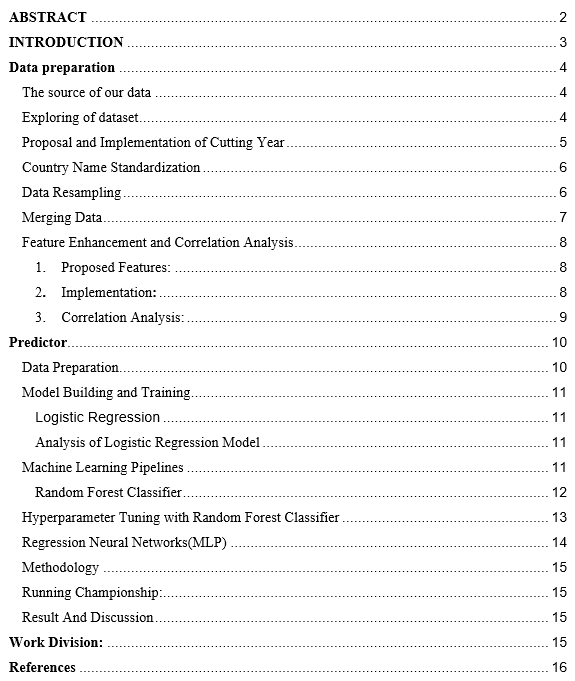
\includegraphics[width=0.75\textwidth]{2023-12-08 165015.png}

	\label{fig:neural_network}
\end{figure}

\newpage
	\section*{Abstract}
	The project aims to build a football match results predictor using machine learning techniques. The focus is on data preparation, feature engineering, and the implementation of regression models to predict match outcomes and championship cup finalists' probabilities. The project involves handling datasets on international football results and FIFA rankings, addressing issues like inconsistent country names, resampling data, and merging datasets. Features such as average goals, points, and rank changes are proposed and added to the model. A correlation analysis is performed to select relevant features. The final step includes optimizing parameters for Random Forest (RF) and Neural Network (NN) models, evaluating their performances, and applying them to championship cup simulations with group and knockout stages. The output provides probabilities for teams to win individual matches and predicts finalists in championship cups.
	
	\newpage % Move to the next page
	
	\section*{Introduction}
	The "Football Match Results Predictor" project is a data-driven exploration focused on predicting outcomes in international football matches and championship cups using machine learning. The initiative begins by preprocessing international football results and FIFA rankings datasets, applying techniques such as resampling, cleaning, and merging. The integrated dataset, named "rera," becomes the foundation for feature engineering, where new variables like average goals and rank changes are introduced. Regression models, specifically Random Forest (RF) and Neural Network (NN), are implemented and fine-tuned using GridSearchCV to optimize parameters. The project evaluates model performance through metrics like confusion matrices and selects the most effective one.
	
	The scope extends to championship cup simulations, covering both group and knockout stages. The project provides insights into the tournament structure, point systems, and match outcomes. Ultimately, the output includes probabilities for individual match results and forecasts the finalist teams in championship cups.
	
	In essence, the project leverages machine learning techniques to enhance football match result predictions, offering a comprehensive framework for understanding and simulating championship cup outcomes.
	
	\newpage % Move to the next page
	
	\section*{Data Preparation}
	\subsection*{The Source of Our Data}
	In the initial phase of our analysis, we loaded two datasets, namely "International Football Results" and "FIFA World Rankings," downloaded from Kaggle. The primary focus was on examining the structures and contents of these datasets. A crucial aspect of this examination involved analyzing country names and identifying commonalities and discrepancies between the two datasets. Noteworthy findings included variations in country names over time, underscoring the importance of harmonizing this information for a comprehensive analysis.
	
	\subsection*{Exploration of the Dataset}
	The provided datasets on FIFA World Rankings (1992-2023) and International Football Results (1872-2023) offer a comprehensive analysis with rich insights into the dynamics of global football. The FIFA World Ranking dataset, anchored by key attributes such as country full name, rank, and confederation, enables a detailed examination of the shifting landscape in international football competitiveness over the past three decades. Notably, the inclusion of rank changes and total points provides a nuanced understanding of each country's performance evolution.\\
	Complementing this, the International Football Results dataset offers a historical perspective with 45,315 recorded matches, ranging from iconic FIFA World Cup clashes to friendly encounters. The dataset captures match details, including scores, tournament names, and venue information, facilitating a deep dive into the evolution of football over time. Combining these datasets presents an opportunity to correlate team performance trends with their FIFA rankings, uncovering patterns and anomalies that contribute to a holistic narrative of international football history.\\
	The data provides a robust foundation for exploring the intricacies of team dynamics, tournament outcomes, and the broader context of global football's evolution.
	\begin{figure}[h]
		\centering
		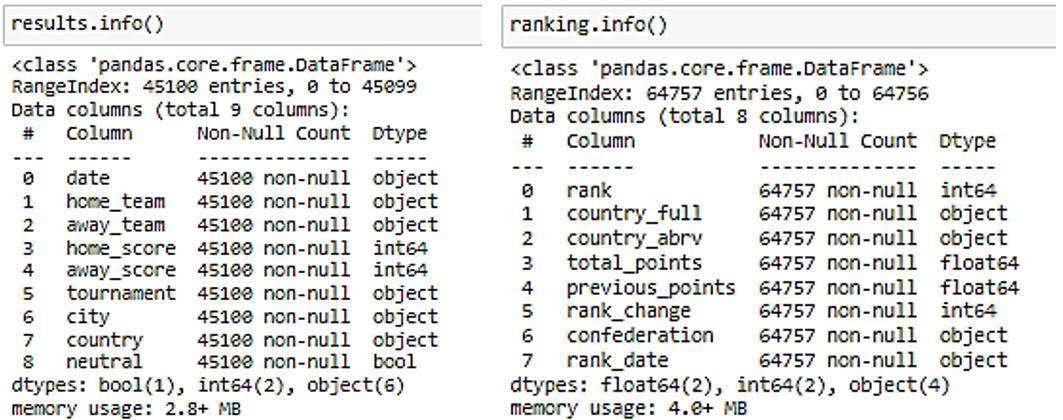
\includegraphics[width=0.8\textwidth]{2023-12-08 150001.png}
		\caption{Ranking and Results Datasets information.}
		\label{fig:neural_network}
	\end{figure}
	\newpage % Move to the next page
	
	\subsection*{Proposal and Implementation of Cutting Year}
	In opting for 2003 as the Cutting year for our analysis, several considerations underscore the approach to maintaining coherence and uniformity across the datasets. The choice is primarily rooted in data availability, as the ranking dataset incorporates information on Serbia only from the close of 2002, necessitating a starting point that ensures the inclusion of the entirety of available Serbian data. Acknowledging the historical significance of events like the dissolution of the Soviet Union in 1992, the decision prioritizes the practicality of handling available data over strict historical alignment. Moreover, starting from 2003, the stabilization of country nomenclature in both datasets enhances consistency, mitigating the risk of discrepancies and facilitating a more seamless correlation of insights. This methodical approach aligns with the temporal availability of the data, fostering a robust and uniform analysis that enhances the reliability of the derived insights across all represented countries, including Serbia.\\
	
	\begin{center}
		\begin{table}[h]
			\centering
		
			\resizebox{0.7\textwidth}{!}{
				\begin{tabular}{|c|c|c|}
					\hline
					Dataset & Original Entries & After Cutting Year \\
					\hline
					Results & 45,100 & 19,477 \\
					Ranking & 64,757 & 45,575 \\
					\hline
				\end{tabular}
				
			}	\caption{Dataset Entries Before and After Cutting Year}
		\end{table}
	\end{center}
	
	\newpage % Move to the next page
	
	\subsection*{Country Name Standardization}
	In addressing inconsistencies within the datasets, a meticulous mapping strategy, as exemplified in the `country name mappings` dictionary, was employed to tackle varied representations of country names. Instances of duplications, such as "Cabo Verde" and "Cape Verde Islands," or variations like "St Kitts and Nevis" versus "St. Kitts and Nevis," were systematically rectified to maintain a single, standardized name for each country. For instance, "Cabo Verde" was homogenized to "Republic of Cabo Verde," ensuring uniformity. Further, the mapping facilitated the transition from "St. Kitts and Nevis" to the standardized "Saint Kitts and Nevis" across both datasets. To illustrate, this approach rectified discrepancies in the representation of "Saint Kitts and Nevis" to ensure consistency between the 'results' and 'ranking' datasets. Post-standardization, a symmetric difference analysis was conducted on the 'FIFA World Cup' matches within the 'results' dataset, resulting in a total of 320 entries. This process exemplifies the dedication to data integrity, as exemplified by the meticulous correction of naming variations, paving the way for robust analyses and model training that hinge on uniform and coherent datasets.
	
	\subsection*{Data Resampling}
	To ensure a seamless integration of ranking data into the results database, a crucial step involved resampling the ranking dataset on a daily basis. The primary challenge arose from the asynchronous nature of data collection, leading to non-coinciding dates between the two databases. By employing Pandas' resampling capabilities, the ranking data was upsampled to daily frequency. This operation resulted in the generation of numerous new rows, each representing a specific day for every country. It's important to note that this process inherently introduced missing data, and to address this, Pandas' `fillna` method was strategically applied. This method intelligently filled in the gaps, ensuring continuity in the time series. Specifically, the 'ffill' (forward fill) approach was adopted, propagating the last valid observation forward to fill the missing values. The resampled and filled ranking data was then meticulously filtered to include only countries present in both the ranking and results datasets, ensuring coherence and completeness in the subsequent analyses.
	
	\begin{figure}[h]
		\centering
		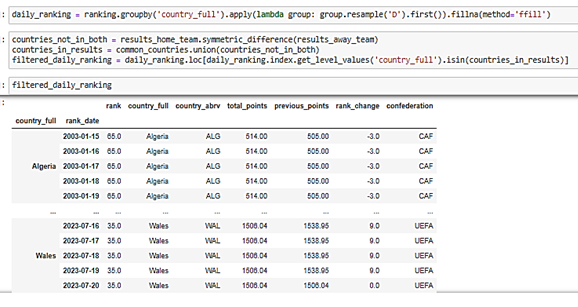
\includegraphics[width=0.8\textwidth]{Picture3.png}
		\caption{ Resampled Dataset.}
		\label{fig:neural_network}
	\end{figure}
	
	\newpage % Move to the next page
	
	\subsection*{Merging Data}
	The integration of ranking data into the results dataset was accomplished through the creation of a consolidated DataFrame named 'rera.' This merging process involved associating each row in the 'results' dataset with corresponding columns from the resampled ranking dataset, encompassing total points, previous points, rank, and rank change for both the home and away teams. The 'rera' DataFrame now encapsulates a comprehensive view of football match data, including relevant attributes such as match date, home and away team names, scores, tournament details, and geographic information. With the successful completion of this merging operation, 'rera' stands as a unified and enriched dataset, laying the groundwork for in-depth analyses and subsequent model training where a holistic view of both match outcomes and team rankings is crucial. The resulting DataFrame exhibits a coherent structure with 320 entries and 17 columns, providing a consolidated and organized foundation for further exploration and insights.\\\\
	\begin{figure}[h]
		\centering
		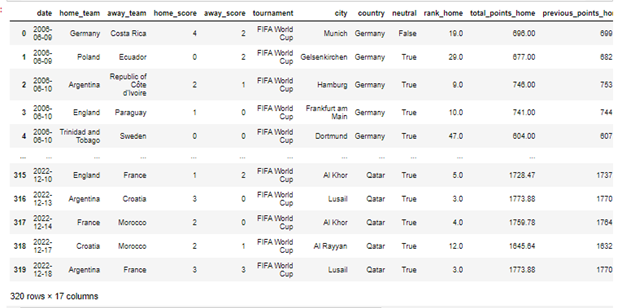
\includegraphics[width=0.8\textwidth]{Picture4.png}
		\caption{ rera dataset.}
		\label{fig:neural_network}
	\end{figure}
	\newpage
	\subsection*{Feature Enhancement and Correlation Analysis }
	
		\subsubsection*{	Proposed Features:}
		This feature calculates the average number of goals scored by a team in their last five matches, providing insights into their recent offensive performance.\\
		
		•	Average Points in Last 5 Matches:\\
		This feature computes the average points earned by a team in their last five matches, considering win, loss, or draw outcomes. It offers a holistic view of the team's recent overall performance.\\
		
		•	Rank Increase During Last 5 Matches:\\
		This feature measures the change in a team's FIFA ranking over the course of their last five matches, providing information on their ranking dynamics and recent competitiveness.\\
		
		•	Average Points in Last 5 Direct Matches:\\
		This feature evaluates the average points earned by a team in their last five direct encounters with another specific team. It offers insights into the team's historical performance against a particular opponent.\\

		\subsubsection*{	Implementation:}
		To incorporate these features into the dataset, Python code was implemented, leveraging Pandas functionalities. The proposed features were added to the 'rera' DataFrame in a consistent manner, enhancing the dataset's richness and providing additional dimensions for predictive modeling.\newpage
		\subsubsection*{	Correlation Analysis:}
		The correlation analysis reveals significant patterns among the features. Strong positive correlations, nearing 1, are identified, such as between 'total points home' and previous points home (0.998811006) and total points away and previous points away (0.998665481). Conversely, robust negative correlations, close to -1, are evident, like those between rank home and both total points home (-0.500838337) and previous points home (-0.503528607), with similar patterns for away teams. To address multicollinearity, it is advised to retain only one feature from each negatively correlated pair. Moreover, intriguing correlations, demanding further exploration, are noted. However, correlations with the target variables (home score and away score) are relatively weak, indicating a limited linear relationship.\\\\
		
			\begin{figure}[h]
			\centering
			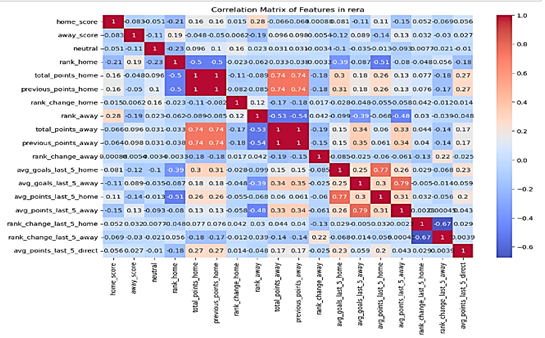
\includegraphics[width=0.8\textwidth]{Picture5.png}
			\caption{  Correlation Matrix.}
			\label{fig:neural_network}
		\end{figure}
		
		\newpage 
		
	\section*{Predictor}	
		\subsection*{Data Preparation}
		The initial phase of data processing involves creating a refined dataset for analysis. To achieve this, we generate a copy of the original dataset, "rera," and create a new DataFrame named 'df.' We strategically eliminate irrelevant columns such as 'Unnamed: 0,' 'date,' 'home team,' and 'away team' to focus on key features for model training. This targeted approach ensures that the dataset is tailored to the specific requirements of our analysis, enhancing the efficiency of subsequent operations.\\\\
		Addressing missing data is a critical aspect of data integrity. Utilizing the SimpleImputer from scikit-learn, we systematically fill missing values in numerical columns with their respective means. This meticulous imputation process maintains the overall dataset consistency, a pivotal prerequisite for accurate model training and evaluation.\\\\
		Following data preparation, we transition to the segmentation phase, where we divide the dataset into feature variables (X) and the target variable (y), with 'win by' identified as our target. Subsequently, we further partition the data into training and testing sets using the train test split function. This strategic split ensures that the model is trained on one subset and tested on another, providing a robust evaluation of its generalization performance.
		Imputation and scaling play a pivotal role in data refinement. The SimpleImputer is reapplied to handle missing values, ensuring both training and testing sets are devoid of gaps in numerical data. StandardScaler is then employed to standardize the features, mitigating the impact of differing scales among variables and contributing to the stability and effectiveness of subsequent machine learning algorithms.
		
		\newpage
		\subsection*{Model Building and Training}
			\subsubsection*{Logistic Regression}
		With the data prepared and missing values handled, the next step involves constructing and training the machine learning model. In this case, a logistic regression model is chosen due to its effectiveness in classification tasks. The logistic regression model is implemented using scikit-learn's LogisticRegression class, with specified parameters such as multi class='multinomial', solver='lbfgs', and a random state of 42 for reproducibility. The training process involves fitting the logistic regression model to the scaled training data. This is achieved by applying the SimpleImputer to impute missing values and the StandardScaler to standardize the features. The imputed and scaled training data is then used to train the logistic regression model.\\
		Once the model is trained, predictions are made on the scaled test set using the predict method. Subsequently, the accuracy of the model is evaluated using the accuracy score function from scikit-learn, comparing the predicted values against the actual target values in the test set.
	
		
			\subsubsection*{Analysis of Logistic Regression Model}
			The analysis of various predictive models for football match outcomes reveals distinct strengths and performance metrics. The logistic regression model demonstrates exceptional accuracy of 98.44\%, showcasing its reliability in predicting match results, particularly for home and away team victories. The Random Forest Classifier, with an accuracy of 89.06\%, exhibits commendable performance, especially in accurately classifying home team victories. The RandomForestRegressor, after hyperparameter tuning, achieves an accuracy of 92.19\%, indicating its effectiveness in predicting the 'win by' variable with consistent precision and recall. Lastly, the Neural Network Regressor, despite facing challenges with the limited dataset, provides valuable insights with an accuracy of 41.98\%, emphasizing the need for further exploration with larger datasets to enhance its predictive capabilities. Each model offers unique strengths, and the choice depends on specific goals and the nature of the prediction task.
		
			\subsubsection*{Machine Learning Pipelines}
			Our analysis hinges on the strategic implementation of Machine Learning Pipelines, robust frameworks that seamlessly navigate data preprocessing, model training, and evaluation. These pipelines showcase their versatility by accommodating both classification and regression tasks. Initiating with a logistic regression model, our pipeline ensures systematic handling of data, addressing missing values, and scaling features. The integration of a Random Forest Classifier further exemplifies the pipeline's adaptability, optimizing model configurations through GridSearchCV. Expanding our pipeline's capabilities to regression tasks, we introduce a Neural Network Regressor, adept at handling challenges posed by limited data. Evaluation metrics, including mean squared error, provide insights into model performance. Crucially, our report emphasizes the scalability and reproducibility of machine learning endeavors through the serialization of models using joblib. In summary, Machine Learning Pipelines emerge as pivotal orchestrators, enhancing collaboration, scalability, and efficiency in constructing and optimizing machine learning models.
		\newpage
		\subsubsection*{Random Forest Classifier}
			Random Forest is an ensemble learning method that constructs a multitude of decision trees during training and outputs the mode of the classes 'classification' or the mean prediction 'regression' of the individual trees. In this specific implementation, the RandomForestClassifier is configured with various hyperparameters such as the number of trees 'n estimators', maximum depth of the trees 'max depth', minimum samples required to split an internal node 'minsamples split', and others. The classifier is integrated into a pipeline that includes a data imputation step using SimpleImputer. The pipeline is then fitted to the training data, enabling the model to learn patterns from the input features. Subsequently, the trained model is used to make predictions on the test set, and the accuracy of the predictions is evaluated using the 'accuracy score' metric.\\\\
			\begin{figure}[h]
				\centering
				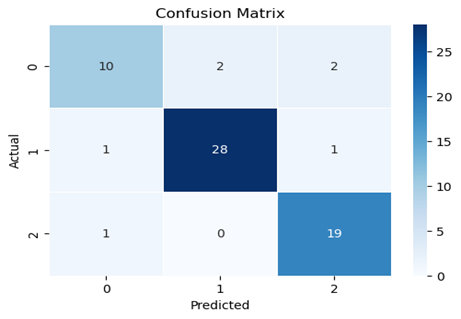
\includegraphics[width=0.8\textwidth]{Picture6.png}
				\caption{ confusion latrix before hyper parameter tunning.}
				\label{fig:neural_network}
			\end{figure}\\	
			The model achieved an accuracy of 89.06\%, demonstrating strong overall performance. The precision, recall, and F1-score metrics provide detailed insights into class-specific performance. Class 1 shows the highest scores, indicating excellent precision (93\%) and recall (93\%), while Class 0 has lower precision (83\%) and recall (71\%). Class 2 exhibits good precision (86\%) and high recall (95\%). The confusion matrix further illustrates the model's ability, showing correct classifications and misclassifications. Overall, the model performs well across multiple metrics, with some variations in performance among different classes.	
			\newpage
		\subsection*{Hyperparameter Tuning with Random Forest Classifier}
		In the Hyperparameter Tuning phase for the Random Forest Classifier, we construct a pipeline that includes critical preprocessing steps like imputation and scaling. The objective is to fine-tune the model's hyperparameters for optimal performance. Using GridSearchCV, we systematically explore hyperparameter combinations, seeking the set that maximizes accuracy. After fitting the GridSearchCV to the training data, we extract and print the best hyperparameters. Evaluation on the test set follows, computing accuracy, mean squared error, a classification report, and a confusion matrix.\\\\
		
		\begin{figure}[h]
			\centering
			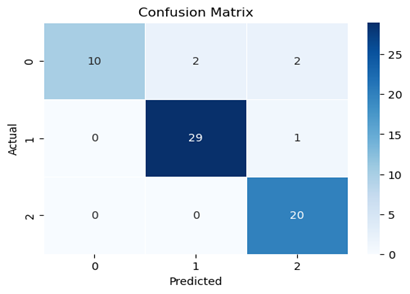
\includegraphics[width=0.8\textwidth]{Picture7.png}
			\caption{ confusion matrix after hyper parameter tuning using grid search cv.}
			\label{fig:neural_network}
		\end{figure}
		
		The model achieved an accuracy of 92.2\% with the best-tuned parameters obtained from GridSearchCV. The precision, recall, and F1-score metrics indicate excellent performance across all classes. Class 0 has perfect precision and high recall, suggesting accurate identification with a slight trade-off in recall. Class 1 exhibits high precision and recall, indicating precise and comprehensive identification. Class 2 showcases perfect precision and recall, highlighting accurate and complete detection. The confusion matrix further validates the model's effectiveness, with minimal misclassifications. Overall, the model demonstrates robust performance, particularly in correctly predicting outcomes for classes 1 and 2, leading to the high accuracy observed.
		
		\newpage
		\subsection*{Regression Neural Networks(MLP)}
		Machine learning pipeline is constructed to train an MLPRegressor (Multi-layer Perceptron Regressor) using a grid search approach for hyperparameter tuning. The data, loaded from the 'rera.csv' file, undergoes preprocessing by dropping unnecessary columns. The feature and target variable separation is followed by splitting the dataset into training and testing sets. The pipeline comprises a StandardScaler for feature scaling, a SimpleImputer for handling missing values, and the MLPRegressor for regression tasks. A hyperparameter grid is defined for the grid search, encompassing parameters such as hidden layer sizes, activation functions, and regularization strength. The GridSearchCV object is employed to systematically explore the hyperparameter space and identify the best combination based on negative mean squared error as the scoring metric. The fitted grid search provides the optimal parameters and the corresponding model accuracy. The best model is then evaluated on the test set, and the mean squared error is computed as a performance metric.
		
		\begin{figure}[h]
			\centering
			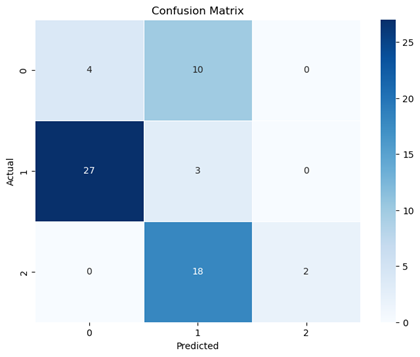
\includegraphics[width=0.8\textwidth]{Picture8.png}
			\caption{ }
			\label{fig:neural_network}
		\end{figure}
		The best model, identified with tanh activation, alpha of 0.01, and a hidden layer size of (50,), achieved an accuracy of approximately 41.98\% and a mean squared error of 0.47 on the test set. However, the classification report and confusion matrix reveal challenges in predicting class labels. Notably, class 2 exhibits perfect precision but limited recall, resulting in a higher F1-score. Classes 0 and 1 display relatively low precision, recall, and F1-scores,. The classification report and confusion matrix of the model shows low precision, recall, and F1-score for each class, indicating difficulty in distinguishing between different outcomes.
		\newpage
	\section*{Methodology}
		The project methodology involves initial data loading and examination of two football-related datasets, followed by an analysis of country names and data preprocessing steps, including feature removal, imputation, and scaling. Logistic regression and Random Forest models are introduced, with the latter undergoing hyperparameter tuning. The best models from both approaches are serialized for future use. The methodology extends to neural network regression, employing MLPRegressor with hyperparameter tuning. The serialized models provide practical deployment options. The relevance of each model is integrated into the broader context of analyzing international football results and FIFA world rankings.
		
	\section*{Running Championship}
		The function runChampionShip serves as the backbone for orchestrating a championship tournament, exhibiting a well-organized and modular design. It commences by establishing the necessary infrastructure, creating a championship file, and initializing folders and files for group stage matches. As it progresses through the tournament workflow, the function seamlessly executes group stage matches, updates points tables, and then seamlessly transitions into a loop iterating four times for simulating knockout rounds. Within each iteration, knockout schedules are generated, matches are conducted, and points tables are updated for the corresponding knockout stage. The script culminates in determining the tournament winner, providing a comprehensive and efficient solution for managing the entire championship process. The code's modular structure not only enhances readability but also facilitates easy maintenance and customization of tournament parameters, showcasing a thoughtful approach to code design.
		\section*{Result And Discussion}
		The project employed logistic regression, random forest, and neural network models to predict international football match outcomes. The logistic regression model achieved a remarkable 98.4\% accuracy, while the random forest model  achieved 89\% accuracy, while after hyperparameter tuning, 92.00\% accuracy with robust precision and recall values. The neural network model, though shows a mean squared error of 0.47, faced challenges in classifying outcomes due to short data. Model serialization enabled us to easily deploy the model and run the championship to get the winner. The methodology involved systematic ML pipelines, hyperparameter tuning, and iterative model exploration. Future considerations include obtaining more data for neural networks and exploring advanced architectures. Overall, the project provides insights into football result prediction, with identified areas for improvement and future analyses.
		\section*{Work Division}
			Muahmmad Ahmed :  preprocessing of data\\
			Dheeraj Parkash : Model Trainings and ml pipelines, to get trained models for prediction\\
			Alireza and Dheeraj Parkash: planning and coding  on working of Championship  \\
			AliReza: Documentation\\
		
		\newpage
	\section*{References}
			DataFrame. (n.d.). From Pandas.: $https://pandas.pydata.org/pandas-docs/stable/reference/api/pandas.DataFrame.html$
			FIFA World Rankings. (n.d.). From FIFA.: $https://www.fifa.com/fifa-world-ranking/ranking-table/men/$
			fifaworldranking. (n.d.). From kaggle: $https://www.kaggle.com/datasets/cashncarry/fifaworldranking$
			Grid Search CV. (n.d.). From Scikit-learn.: $https://scikit-learn.org/stable/modules/generated/sklearn.model_selection.GridSearchCV.html$
			$https://www.kaggle.com/martj42/international-football-results-from-1872-to-2017.$ (n.d.). Kaggle Dataset. From International Football Results.
			Joblib. (n.d.). From Joblib.: $https://joblib.readthedocs.io/en/latest/
			Logistic Regression.$ (n.d.). From Scikit-learn.: $https://scikit-learn.org/stable/modules/generated/sklearn.linear_model.LogisticRegression.html
			MLP Regressor.$ (n.d.). From Scikit-learn.: $https://scikit-learn.org/stable/modules/generated/sklearn.neural_network.MLPRegressor.html$
			Pipeline. (n.d.). From Scikit-learn.: $https://scikit-learn.org/stable/modules/generated/sklearn.pipeline.Pipeline.html$
			Pyplot. (n.d.). From Matplotlib.: $https://matplotlib.org/stable/api/pyplot_summary.html$
			Random Forest Classifier. (n.d.). From Scikit-learn.: $https://scikit-learn.org/stable/modules/generated/sklearn.ensemble.RandomForestClassifier.html$
			Seaborn. (n.d.). From Seaborn.: $https://seaborn.pydata.org/$
		
		
		
\end{document}
